\documentclass[twoside]{book}

% Packages required by doxygen
\usepackage{fixltx2e}
\usepackage{calc}
\usepackage{doxygen}
\usepackage[export]{adjustbox} % also loads graphicx
\usepackage{graphicx}
\usepackage[utf8]{inputenc}
\usepackage{makeidx}
\usepackage{multicol}
\usepackage{multirow}
\PassOptionsToPackage{warn}{textcomp}
\usepackage{textcomp}
\usepackage[nointegrals]{wasysym}
\usepackage[table]{xcolor}

% Font selection
\usepackage[T1]{fontenc}
\usepackage[scaled=.90]{helvet}
\usepackage{courier}
\usepackage{amssymb}
\usepackage{sectsty}
\renewcommand{\familydefault}{\sfdefault}
\allsectionsfont{%
  \fontseries{bc}\selectfont%
  \color{darkgray}%
}
\renewcommand{\DoxyLabelFont}{%
  \fontseries{bc}\selectfont%
  \color{darkgray}%
}
\newcommand{\+}{\discretionary{\mbox{\scriptsize$\hookleftarrow$}}{}{}}

% Page & text layout
\usepackage{geometry}
\geometry{%
  a4paper,%
  top=2.5cm,%
  bottom=2.5cm,%
  left=2.5cm,%
  right=2.5cm%
}
\tolerance=750
\hfuzz=15pt
\hbadness=750
\setlength{\emergencystretch}{15pt}
\setlength{\parindent}{0cm}
\setlength{\parskip}{3ex plus 2ex minus 2ex}
\makeatletter
\renewcommand{\paragraph}{%
  \@startsection{paragraph}{4}{0ex}{-1.0ex}{1.0ex}{%
    \normalfont\normalsize\bfseries\SS@parafont%
  }%
}
\renewcommand{\subparagraph}{%
  \@startsection{subparagraph}{5}{0ex}{-1.0ex}{1.0ex}{%
    \normalfont\normalsize\bfseries\SS@subparafont%
  }%
}
\makeatother

% Headers & footers
\usepackage{fancyhdr}
\pagestyle{fancyplain}
\fancyhead[LE]{\fancyplain{}{\bfseries\thepage}}
\fancyhead[CE]{\fancyplain{}{}}
\fancyhead[RE]{\fancyplain{}{\bfseries\leftmark}}
\fancyhead[LO]{\fancyplain{}{\bfseries\rightmark}}
\fancyhead[CO]{\fancyplain{}{}}
\fancyhead[RO]{\fancyplain{}{\bfseries\thepage}}
\fancyfoot[LE]{\fancyplain{}{}}
\fancyfoot[CE]{\fancyplain{}{}}
\fancyfoot[RE]{\fancyplain{}{\bfseries\scriptsize Generated by Doxygen }}
\fancyfoot[LO]{\fancyplain{}{\bfseries\scriptsize Generated by Doxygen }}
\fancyfoot[CO]{\fancyplain{}{}}
\fancyfoot[RO]{\fancyplain{}{}}
\renewcommand{\footrulewidth}{0.4pt}
\renewcommand{\chaptermark}[1]{%
  \markboth{#1}{}%
}
\renewcommand{\sectionmark}[1]{%
  \markright{\thesection\ #1}%
}

% Indices & bibliography
\usepackage{natbib}
\usepackage[titles]{tocloft}
\setcounter{tocdepth}{3}
\setcounter{secnumdepth}{5}
\makeindex

% Hyperlinks (required, but should be loaded last)
\usepackage{ifpdf}
\ifpdf
  \usepackage[pdftex,pagebackref=true]{hyperref}
\else
  \usepackage[ps2pdf,pagebackref=true]{hyperref}
\fi
\hypersetup{%
  colorlinks=true,%
  linkcolor=blue,%
  citecolor=blue,%
  unicode%
}

% Custom commands
\newcommand{\clearemptydoublepage}{%
  \newpage{\pagestyle{empty}\cleardoublepage}%
}

\usepackage{caption}
\captionsetup{labelsep=space,justification=centering,font={bf},singlelinecheck=off,skip=4pt,position=top}

%===== C O N T E N T S =====

\begin{document}

% Titlepage & ToC
\hypersetup{pageanchor=false,
             bookmarksnumbered=true,
             pdfencoding=unicode
            }
\pagenumbering{alph}
\begin{titlepage}
\vspace*{7cm}
\begin{center}%
{\Large nasteroids }\\
\vspace*{1cm}
{\large Generated by Doxygen 1.8.13}\\
\end{center}
\end{titlepage}
\clearemptydoublepage
\pagenumbering{roman}
\tableofcontents
\clearemptydoublepage
\pagenumbering{arabic}
\hypersetup{pageanchor=true}

%--- Begin generated contents ---
\chapter{nasteroids}
\label{md__r_e_a_d_m_e}
\Hypertarget{md__r_e_a_d_m_e}
\href{https://travis-ci.com/RaulOlmedoCheca/nasteroids}{\tt } \href{https://www.codacy.com?utm_source=github.com&amp;utm_medium=referral&amp;utm_content=RaulOlmedoCheca/nasteroids&amp;utm_campaign=Badge_Grade}{\tt }

Final Project of A\+R\+C\+OS

\subsection*{T\+O\+DO\+:}

\subsection*{Documentation}

\subsubsection*{Parameters of the program\+:}

{\bfseries num\+\_\+asteroids\+:} is an integer number, greater or equal than 0, which indicates the number of asteroids that will be simulated.

{\bfseries num iterations\+:} is an integer number, greater or equal than 0, which indicates the number of iterations (time steps) that will be simulated.

{\bfseries num\+\_\+planets\+:} is an integer number, greater or equal than 0, which indicates the number of planets that will be included at the border of the space.

{\bfseries pos\+\_\+ray\+:} is a double precision floating point number, which indicates the exact position of the ray in the space (y coordinate).

{\bfseries seed\+:} is a positive integer number that serves as seed for the generator functions for random numbers.

\subsubsection*{Calling the program}

{\ttfamily nasteroids-\/seq num\textbackslash{}\+\_\+asteroids num\textbackslash{}\+\_\+iterations num\textbackslash{}\+\_\+planets pos\textbackslash{}\+\_\+ray seed}

\subsubsection*{Generated output}

{\ttfamily init\+\_\+config.\+txt} containing\+:


\begin{DoxyItemize}
\item Input parameters separated by a space in the same order in which they were introduced (without including the name of the program).
\item For each asteroid first, planet and ray, their position must be stored (x and y), as well as their mass (only for asteroids). Each element must be written in a line wit their parameters separated by spaces. When printing floating point numbers, 3 decimals must be printed.
\end{DoxyItemize}


\begin{DoxyCode}
\textcolor{comment}{// Random distributions}
default\_random\_engine re\{seed\};
uniform\_real\_distribution<double> xdist\{0.0, std::nextafter(width, std::numeric\_limits<double>::max())\};
uniform\_real\_distribution<double> ydist\{0.0, std::nextafter(height, std::numeric\_limits<double>::max())\};
normal\_distribution<double> mdist\{mass, sdm\};
\end{DoxyCode}
 
\chapter{Hierarchical Index}
\section{Class Hierarchy}
This inheritance list is sorted roughly, but not completely, alphabetically\+:\begin{DoxyCompactList}
\item \contentsline{section}{Body}{\pageref{class_body}}{}
\begin{DoxyCompactList}
\item \contentsline{section}{Asteroid}{\pageref{class_asteroid}}{}
\item \contentsline{section}{Planet}{\pageref{class_planet}}{}
\end{DoxyCompactList}
\end{DoxyCompactList}

\chapter{Class Index}
\section{Class List}
Here are the classes, structs, unions and interfaces with brief descriptions\+:\begin{DoxyCompactList}
\item\contentsline{section}{\hyperlink{class_asteroid}{Asteroid} }{\pageref{class_asteroid}}{}
\item\contentsline{section}{\hyperlink{class_body}{Body} }{\pageref{class_body}}{}
\item\contentsline{section}{\hyperlink{class_planet}{Planet} }{\pageref{class_planet}}{}
\end{DoxyCompactList}

\chapter{Class Documentation}
\hypertarget{class_asteroid}{}\section{Asteroid Class Reference}
\label{class_asteroid}\index{Asteroid@{Asteroid}}
Inheritance diagram for Asteroid\+:\begin{figure}[H]
\begin{center}
\leavevmode
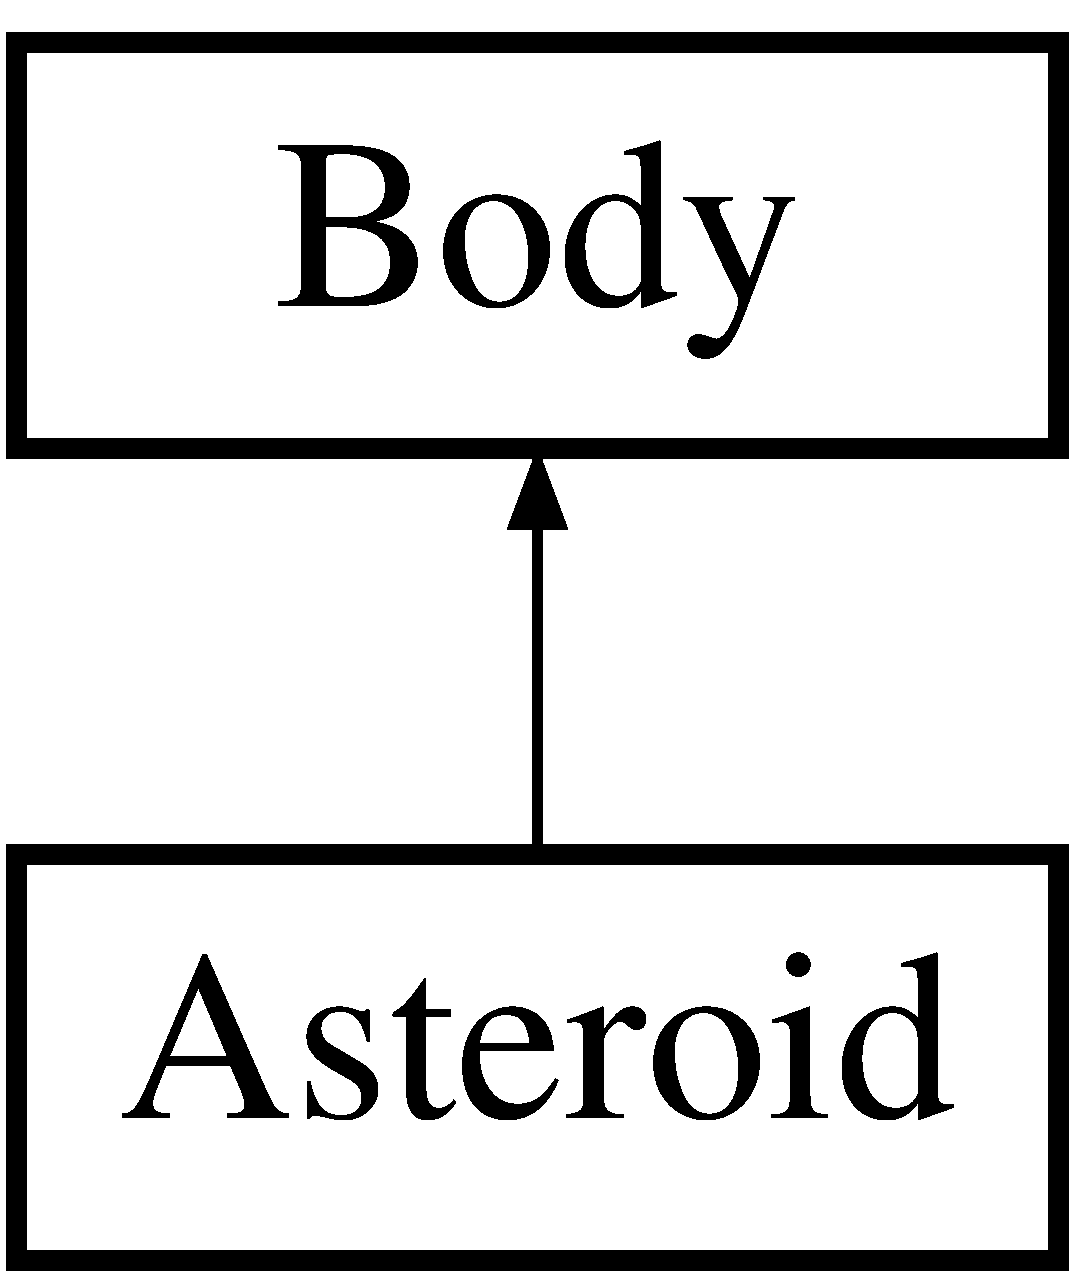
\includegraphics[height=2.000000cm]{class_asteroid}
\end{center}
\end{figure}
\subsection*{Public Member Functions}
\begin{DoxyCompactItemize}
\item 
void \hyperlink{class_asteroid_add92a2b3252e34bb4565c0d4e0a1ee6d}{set\+VelocityX} (double velocityX)
\item 
void \hyperlink{class_asteroid_a0e915ddddb72eaa3f10f638cd1e567f2}{set\+VelocityY} (double velocityY)
\item 
double \hyperlink{class_asteroid_a193de757c5b2a09dbc60ad5c9e973cac}{get\+VelocityX} ()
\item 
double \hyperlink{class_asteroid_a2dc08e878983626c16ef45626ffab703}{get\+VelocityY} ()
\item 
\hyperlink{class_asteroid_a3d9a9efa0c313401971e99244c58fa01}{Asteroid} (double posX, double posY, double mass, double velocityX, double velocityY)
\end{DoxyCompactItemize}


\subsection{Constructor \& Destructor Documentation}
\mbox{\Hypertarget{class_asteroid_a3d9a9efa0c313401971e99244c58fa01}\label{class_asteroid_a3d9a9efa0c313401971e99244c58fa01}} 
\index{Asteroid@{Asteroid}!Asteroid@{Asteroid}}
\index{Asteroid@{Asteroid}!Asteroid@{Asteroid}}
\subsubsection{\texorpdfstring{Asteroid()}{Asteroid()}}
{\footnotesize\ttfamily Asteroid\+::\+Asteroid (\begin{DoxyParamCaption}\item[{double}]{posX,  }\item[{double}]{posY,  }\item[{double}]{mass,  }\item[{double}]{velocityX,  }\item[{double}]{velocityY }\end{DoxyParamCaption})}

T\+O\+DO\+: 
\begin{DoxyParams}{Parameters}
{\em posX} & \\
\hline
{\em posY} & \\
\hline
{\em mass} & \\
\hline
{\em velocity} & \\
\hline
\end{DoxyParams}


\subsection{Member Function Documentation}
\mbox{\Hypertarget{class_asteroid_a193de757c5b2a09dbc60ad5c9e973cac}\label{class_asteroid_a193de757c5b2a09dbc60ad5c9e973cac}} 
\index{Asteroid@{Asteroid}!get\+VelocityX@{get\+VelocityX}}
\index{get\+VelocityX@{get\+VelocityX}!Asteroid@{Asteroid}}
\subsubsection{\texorpdfstring{get\+Velocity\+X()}{getVelocityX()}}
{\footnotesize\ttfamily double Asteroid\+::get\+VelocityX (\begin{DoxyParamCaption}{ }\end{DoxyParamCaption})}

T\+O\+DO\+: \begin{DoxyReturn}{Returns}

\end{DoxyReturn}
\mbox{\Hypertarget{class_asteroid_a2dc08e878983626c16ef45626ffab703}\label{class_asteroid_a2dc08e878983626c16ef45626ffab703}} 
\index{Asteroid@{Asteroid}!get\+VelocityY@{get\+VelocityY}}
\index{get\+VelocityY@{get\+VelocityY}!Asteroid@{Asteroid}}
\subsubsection{\texorpdfstring{get\+Velocity\+Y()}{getVelocityY()}}
{\footnotesize\ttfamily double Asteroid\+::get\+VelocityY (\begin{DoxyParamCaption}{ }\end{DoxyParamCaption})}

T\+O\+DO\+: \begin{DoxyReturn}{Returns}

\end{DoxyReturn}
\mbox{\Hypertarget{class_asteroid_add92a2b3252e34bb4565c0d4e0a1ee6d}\label{class_asteroid_add92a2b3252e34bb4565c0d4e0a1ee6d}} 
\index{Asteroid@{Asteroid}!set\+VelocityX@{set\+VelocityX}}
\index{set\+VelocityX@{set\+VelocityX}!Asteroid@{Asteroid}}
\subsubsection{\texorpdfstring{set\+Velocity\+X()}{setVelocityX()}}
{\footnotesize\ttfamily void Asteroid\+::set\+VelocityX (\begin{DoxyParamCaption}\item[{double}]{velocityX }\end{DoxyParamCaption})}

T\+O\+DO\+: 
\begin{DoxyParams}{Parameters}
{\em velocityX} & \\
\hline
\end{DoxyParams}
\mbox{\Hypertarget{class_asteroid_a0e915ddddb72eaa3f10f638cd1e567f2}\label{class_asteroid_a0e915ddddb72eaa3f10f638cd1e567f2}} 
\index{Asteroid@{Asteroid}!set\+VelocityY@{set\+VelocityY}}
\index{set\+VelocityY@{set\+VelocityY}!Asteroid@{Asteroid}}
\subsubsection{\texorpdfstring{set\+Velocity\+Y()}{setVelocityY()}}
{\footnotesize\ttfamily void Asteroid\+::set\+VelocityY (\begin{DoxyParamCaption}\item[{double}]{velocityY }\end{DoxyParamCaption})}

T\+O\+DO\+: 
\begin{DoxyParams}{Parameters}
{\em velocityY} & \\
\hline
\end{DoxyParams}


The documentation for this class was generated from the following files\+:\begin{DoxyCompactItemize}
\item 
Asteroid.\+h\item 
Asteroid.\+cpp\end{DoxyCompactItemize}

\hypertarget{class_body}{}\section{Body Class Reference}
\label{class_body}\index{Body@{Body}}
Inheritance diagram for Body\+:\begin{figure}[H]
\begin{center}
\leavevmode
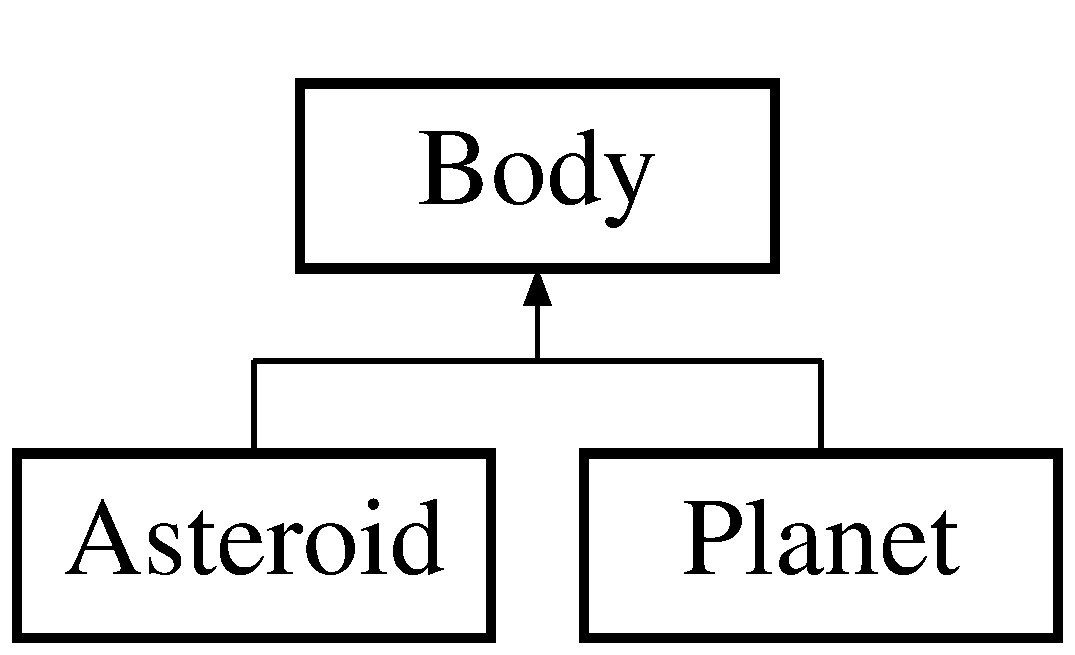
\includegraphics[height=2.000000cm]{class_body}
\end{center}
\end{figure}
\subsection*{Public Member Functions}
\begin{DoxyCompactItemize}
\item 
virtual void \hyperlink{class_body_a14266f71a12e9ccab50afa62c92f57f6}{set\+PosX} (double posX)
\item 
virtual void \hyperlink{class_body_ae2d1b21596116c4d7e863420ea500ac8}{set\+PosY} (double posY)
\item 
double \hyperlink{class_body_aad904543c769a0fa454d2ef9b98c4cd4}{get\+PosX} (void)
\item 
double \hyperlink{class_body_aaa6bdeccdffda065788bf9194fb93a6a}{get\+PosY} (void)
\item 
double \hyperlink{class_body_a3620d6fdf0280daec1c1bf7c75fb4bc4}{get\+Mass} (void)
\item 
\hyperlink{class_body_ac8304d77f5f5b281a54c53e17cb4b4b8}{Body} (double posX, double posY, double mass)
\item 
\hyperlink{class_body_abe1c4da65568cf7978b6247affc461e3}{$\sim$\+Body} ()
\end{DoxyCompactItemize}


\subsection{Constructor \& Destructor Documentation}
\mbox{\Hypertarget{class_body_ac8304d77f5f5b281a54c53e17cb4b4b8}\label{class_body_ac8304d77f5f5b281a54c53e17cb4b4b8}} 
\index{Body@{Body}!Body@{Body}}
\index{Body@{Body}!Body@{Body}}
\subsubsection{\texorpdfstring{Body()}{Body()}}
{\footnotesize\ttfamily Body\+::\+Body (\begin{DoxyParamCaption}\item[{double}]{posX,  }\item[{double}]{posY,  }\item[{double}]{mass }\end{DoxyParamCaption})}

T\+O\+DO\+: 
\begin{DoxyParams}{Parameters}
{\em posX} & \\
\hline
{\em posY} & \\
\hline
{\em mass} & \\
\hline
\end{DoxyParams}
\mbox{\Hypertarget{class_body_abe1c4da65568cf7978b6247affc461e3}\label{class_body_abe1c4da65568cf7978b6247affc461e3}} 
\index{Body@{Body}!````~Body@{$\sim$\+Body}}
\index{````~Body@{$\sim$\+Body}!Body@{Body}}
\subsubsection{\texorpdfstring{$\sim$\+Body()}{~Body()}}
{\footnotesize\ttfamily Body\+::$\sim$\+Body (\begin{DoxyParamCaption}{ }\end{DoxyParamCaption})}

T\+O\+DO\+: 

\subsection{Member Function Documentation}
\mbox{\Hypertarget{class_body_a3620d6fdf0280daec1c1bf7c75fb4bc4}\label{class_body_a3620d6fdf0280daec1c1bf7c75fb4bc4}} 
\index{Body@{Body}!get\+Mass@{get\+Mass}}
\index{get\+Mass@{get\+Mass}!Body@{Body}}
\subsubsection{\texorpdfstring{get\+Mass()}{getMass()}}
{\footnotesize\ttfamily double Body\+::get\+Mass (\begin{DoxyParamCaption}\item[{void}]{ }\end{DoxyParamCaption})}

T\+O\+DO\+: \begin{DoxyReturn}{Returns}

\end{DoxyReturn}
\mbox{\Hypertarget{class_body_aad904543c769a0fa454d2ef9b98c4cd4}\label{class_body_aad904543c769a0fa454d2ef9b98c4cd4}} 
\index{Body@{Body}!get\+PosX@{get\+PosX}}
\index{get\+PosX@{get\+PosX}!Body@{Body}}
\subsubsection{\texorpdfstring{get\+Pos\+X()}{getPosX()}}
{\footnotesize\ttfamily double Body\+::get\+PosX (\begin{DoxyParamCaption}\item[{void}]{ }\end{DoxyParamCaption})}

T\+O\+DO\+: \begin{DoxyReturn}{Returns}

\end{DoxyReturn}
\mbox{\Hypertarget{class_body_aaa6bdeccdffda065788bf9194fb93a6a}\label{class_body_aaa6bdeccdffda065788bf9194fb93a6a}} 
\index{Body@{Body}!get\+PosY@{get\+PosY}}
\index{get\+PosY@{get\+PosY}!Body@{Body}}
\subsubsection{\texorpdfstring{get\+Pos\+Y()}{getPosY()}}
{\footnotesize\ttfamily double Body\+::get\+PosY (\begin{DoxyParamCaption}\item[{void}]{ }\end{DoxyParamCaption})}

T\+O\+DO\+: \begin{DoxyReturn}{Returns}

\end{DoxyReturn}
\mbox{\Hypertarget{class_body_a14266f71a12e9ccab50afa62c92f57f6}\label{class_body_a14266f71a12e9ccab50afa62c92f57f6}} 
\index{Body@{Body}!set\+PosX@{set\+PosX}}
\index{set\+PosX@{set\+PosX}!Body@{Body}}
\subsubsection{\texorpdfstring{set\+Pos\+X()}{setPosX()}}
{\footnotesize\ttfamily void Body\+::set\+PosX (\begin{DoxyParamCaption}\item[{double}]{posX }\end{DoxyParamCaption})\hspace{0.3cm}{\ttfamily [virtual]}}

T\+O\+DO\+: 
\begin{DoxyParams}{Parameters}
{\em posX} & \\
\hline
\end{DoxyParams}


Reimplemented in \hyperlink{class_planet_af7342d2cef15fb89acde2541c2cc678c}{Planet}.

\mbox{\Hypertarget{class_body_ae2d1b21596116c4d7e863420ea500ac8}\label{class_body_ae2d1b21596116c4d7e863420ea500ac8}} 
\index{Body@{Body}!set\+PosY@{set\+PosY}}
\index{set\+PosY@{set\+PosY}!Body@{Body}}
\subsubsection{\texorpdfstring{set\+Pos\+Y()}{setPosY()}}
{\footnotesize\ttfamily void Body\+::set\+PosY (\begin{DoxyParamCaption}\item[{double}]{posY }\end{DoxyParamCaption})\hspace{0.3cm}{\ttfamily [virtual]}}

T\+O\+DO\+: 
\begin{DoxyParams}{Parameters}
{\em posY} & \\
\hline
\end{DoxyParams}


Reimplemented in \hyperlink{class_planet_afb1d37f2f3ce325133604f40ff59c664}{Planet}.



The documentation for this class was generated from the following files\+:\begin{DoxyCompactItemize}
\item 
Body.\+h\item 
Body.\+cpp\end{DoxyCompactItemize}

\hypertarget{class_planet}{}\section{Planet Class Reference}
\label{class_planet}\index{Planet@{Planet}}
Inheritance diagram for Planet\+:\begin{figure}[H]
\begin{center}
\leavevmode
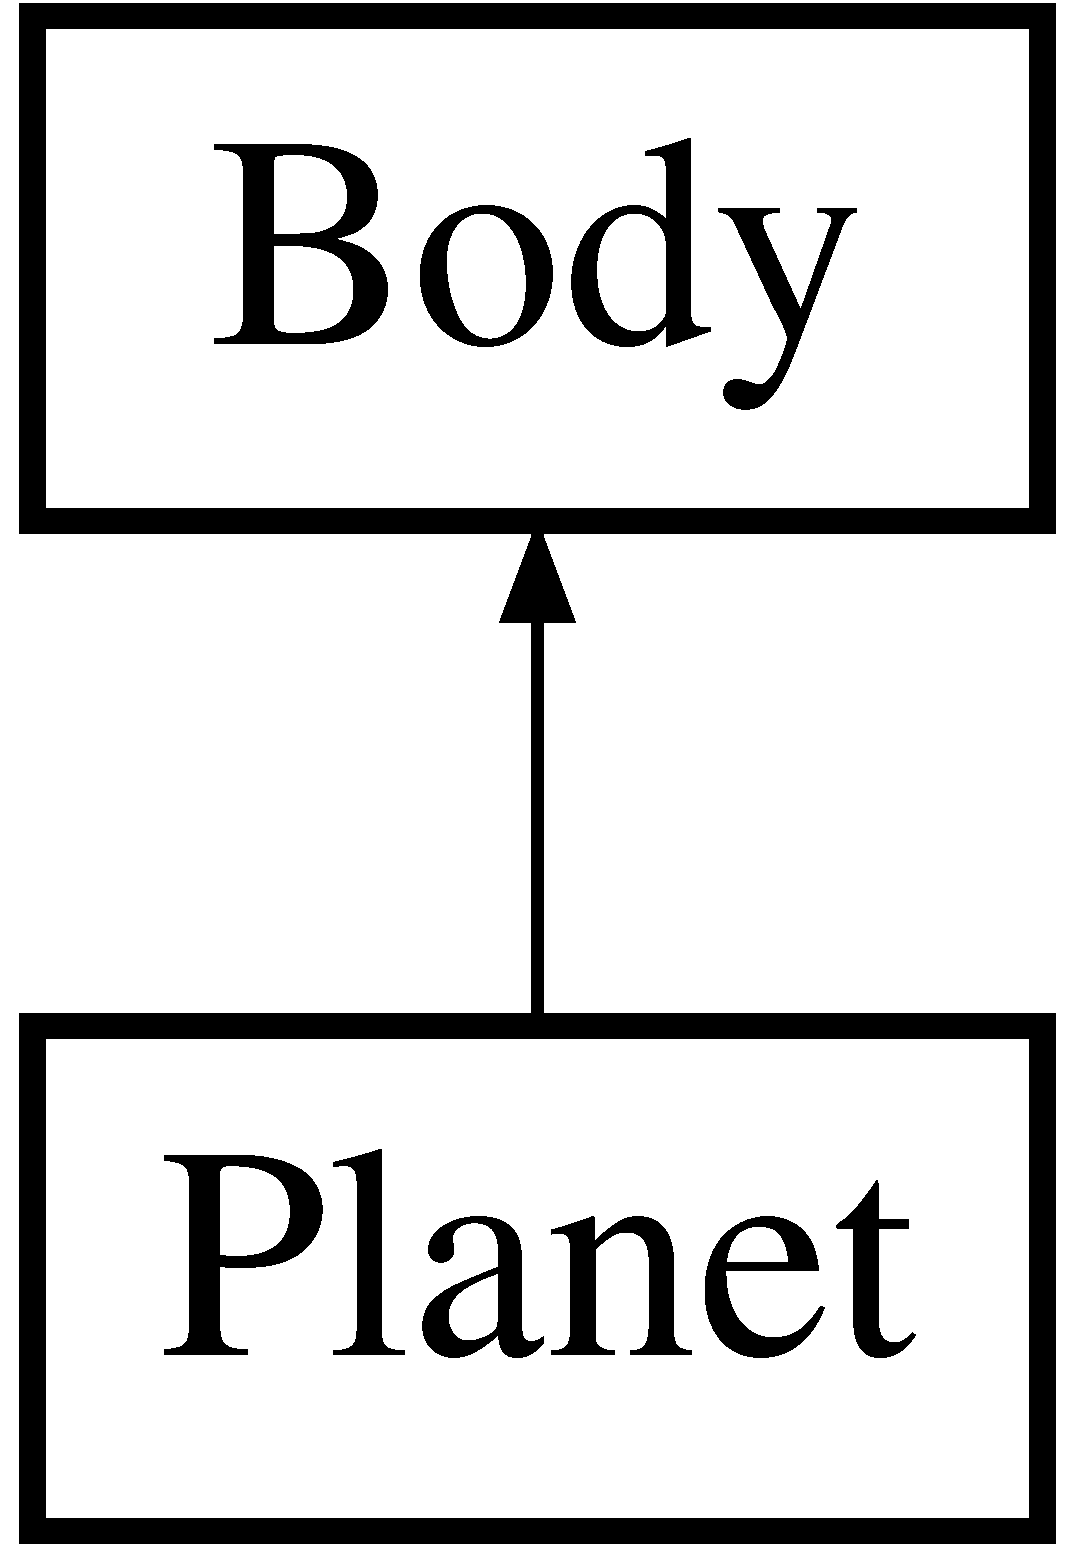
\includegraphics[height=2.000000cm]{class_planet}
\end{center}
\end{figure}
\subsection*{Public Member Functions}
\begin{DoxyCompactItemize}
\item 
void \hyperlink{class_planet_af7342d2cef15fb89acde2541c2cc678c}{set\+PosX} (double posX) override
\item 
void \hyperlink{class_planet_afb1d37f2f3ce325133604f40ff59c664}{set\+PosY} (double posY) override
\item 
\hyperlink{class_planet_a1d2c095a5a90bd9f8719deee853fe178}{Planet} (double posX, double posY, double mass)
\end{DoxyCompactItemize}


\subsection{Constructor \& Destructor Documentation}
\mbox{\Hypertarget{class_planet_a1d2c095a5a90bd9f8719deee853fe178}\label{class_planet_a1d2c095a5a90bd9f8719deee853fe178}} 
\index{Planet@{Planet}!Planet@{Planet}}
\index{Planet@{Planet}!Planet@{Planet}}
\subsubsection{\texorpdfstring{Planet()}{Planet()}}
{\footnotesize\ttfamily Planet\+::\+Planet (\begin{DoxyParamCaption}\item[{double}]{posX,  }\item[{double}]{posY,  }\item[{double}]{mass }\end{DoxyParamCaption})}

T\+O\+DO\+: 
\begin{DoxyParams}{Parameters}
{\em posX} & \\
\hline
{\em posY} & \\
\hline
{\em mass} & \\
\hline
\end{DoxyParams}


\subsection{Member Function Documentation}
\mbox{\Hypertarget{class_planet_af7342d2cef15fb89acde2541c2cc678c}\label{class_planet_af7342d2cef15fb89acde2541c2cc678c}} 
\index{Planet@{Planet}!set\+PosX@{set\+PosX}}
\index{set\+PosX@{set\+PosX}!Planet@{Planet}}
\subsubsection{\texorpdfstring{set\+Pos\+X()}{setPosX()}}
{\footnotesize\ttfamily void Planet\+::set\+PosX (\begin{DoxyParamCaption}\item[{double}]{posX }\end{DoxyParamCaption})\hspace{0.3cm}{\ttfamily [override]}, {\ttfamily [virtual]}}

T\+O\+DO\+: 
\begin{DoxyParams}{Parameters}
{\em posX} & \\
\hline
\end{DoxyParams}


Reimplemented from \hyperlink{class_body_a14266f71a12e9ccab50afa62c92f57f6}{Body}.

\mbox{\Hypertarget{class_planet_afb1d37f2f3ce325133604f40ff59c664}\label{class_planet_afb1d37f2f3ce325133604f40ff59c664}} 
\index{Planet@{Planet}!set\+PosY@{set\+PosY}}
\index{set\+PosY@{set\+PosY}!Planet@{Planet}}
\subsubsection{\texorpdfstring{set\+Pos\+Y()}{setPosY()}}
{\footnotesize\ttfamily void Planet\+::set\+PosY (\begin{DoxyParamCaption}\item[{double}]{posY }\end{DoxyParamCaption})\hspace{0.3cm}{\ttfamily [override]}, {\ttfamily [virtual]}}

T\+O\+DO\+: 
\begin{DoxyParams}{Parameters}
{\em posY} & \\
\hline
\end{DoxyParams}


Reimplemented from \hyperlink{class_body_ae2d1b21596116c4d7e863420ea500ac8}{Body}.



The documentation for this class was generated from the following files\+:\begin{DoxyCompactItemize}
\item 
Planet.\+h\item 
Planet.\+cpp\end{DoxyCompactItemize}

%--- End generated contents ---

% Index
\backmatter
\newpage
\phantomsection
\clearemptydoublepage
\addcontentsline{toc}{chapter}{Index}
\printindex

\end{document}
